\chapter{Results and discussion}

The content of this chapter would be reported as the analysis 
procedure from step one to the end. The first part is the data 
correction process, count maps from the raw count as well as 
exposure map from the parallel computation, the spectrum and 
inversion model fitting by heuristic optimization.

\section{Limb's angle correction}
Theoretically, the peak profile of the $\theta_\text{NADIR}$ would be
the same. From the observations, the of nadir angle change through time 
evolving since the spacecraft altitude is gradually getting lower
in each year which will affect the LAT point of view when it see 
the Earth.

\begin{figure}[h]
    \centering
    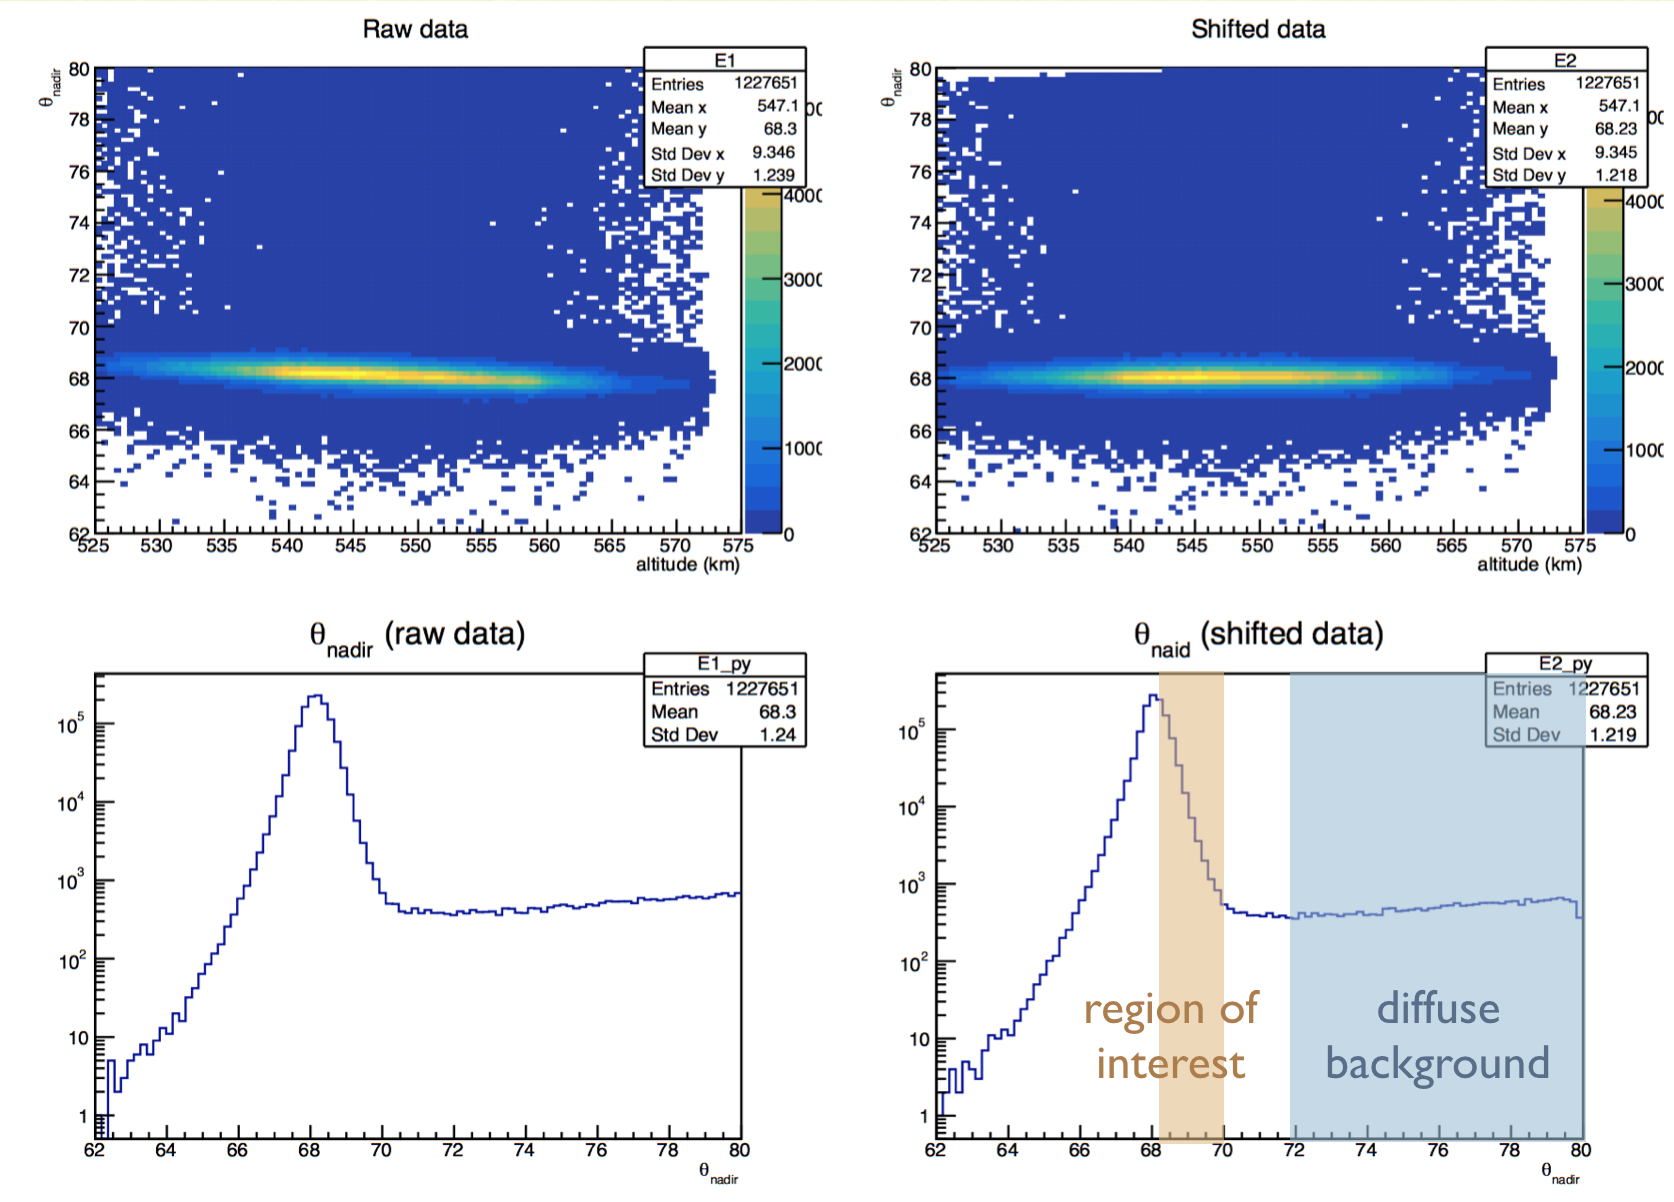
\includegraphics[width=0.8\textwidth]{content/result_and_discussion/figures/LATShifted.png}
    \caption{Distribution of nadir angle before and after altitude correction}
    \label{fig:lat_nadir_shifted}
\end{figure}


The top-left of Figure \ref{fig:lat_nadir_shifted} demonstrates how 
much spacecraft orbitting altitude correlate to the $\theta_\text{NADIR}$
by a 2D heatmap plot of photon intensity. The bottom-left histogram
came from the projection of the previous raw count 2-D histogram which 
has a peak around 68\textdegree. Both bottom and top right histograms
was contructed from exactly same logic but there is one different 
variable. The shifted nadir angle has been calculated to reduce the 
effect from the spacecraft and the region of interest has been highlighed 
as orange for calculating as the limb spectrum and the blue zone is 
a diffusive background to be used in the background substraction.


\section{$\gamma$-ray measurement}


\subsection{}

\section{Best fit result}


\section{Error determination}

